% arara: pdflatex
% !arara: biber
% !arara: pdflatex
% How to run: 
% 1) pdflatex "filename".tex
% 2) biber "filename"
% 3) pdflatex "filename".tex
% 4) pdflatex "filename".tex


\documentclass[x11names]{article}
\usepackage{verbatim}
\usepackage{listings}
\usepackage{graphicx}
\usepackage{a4wide}
\usepackage{color}
\usepackage{amsmath}
\usepackage{amssymb}
\usepackage[dvips]{epsfig}
\usepackage[T1]{fontenc}
% \usepackage{cite} % [2,3,4] --> [2--4]
\usepackage{shadow}
\usepackage{hyperref}
\usepackage{physics}
\usepackage{url}
%For use in pictures
\usepackage{tikz}
\usepackage{tikz-3dplot}
\usepackage{wrapfig}


\usepackage{subcaption}
\usepackage[utf8]{inputenc}
\usepackage{booktabs} % Allows the use of \toprule, \midrule and \bottomrule in tables
\usepackage[font={small,it}]{caption}
\usepackage[margin=0.7in]{geometry} %Sets the margins in the document
\usepackage{siunitx}    %Allows use of SI units macros

%Defines calculator way to write powers of ten
\sisetup{output-exponent-marker=\textsc{e}}


% Change numbering and some commands
\renewcommand\thesection{Exercise \Roman{section}}
\renewcommand\thesubsection{\Roman{section}.\alph{subsection}}

%% references
\usepackage[style=authoryear,
            bibstyle=authoryear,
            backend=biber,
            % refsection=chapter,
            maxbibnames=99,
            maxnames=2,
            firstinits=true,
            uniquename=init,
            natbib=true,
            dashed=false]{biblatex}

\addbibresource{bibliography.bib}
% \addbibresource{top.bib}

% \bibliography{bibliography}
% \bibliography{top}


\usepackage[capitalize]{cleveref}

\setcounter{tocdepth}{2}

\lstset{language=c++}
\lstset{alsolanguage=[90]Fortran}
\lstset{basicstyle=\small}
\lstset{backgroundcolor=\color{white}}
\lstset{frame=single}
\lstset{stringstyle=\ttfamily}
\lstset{keywordstyle=\color{red}\bfseries}
\lstset{commentstyle=\itshape\color{blue}}
\lstset{showspaces=false}
\lstset{showstringspaces=false}
\lstset{showtabs=false}
\lstset{breaklines}


\definecolor{keywords}{RGB}{255,0,90}
      \definecolor{comments}{RGB}{0,0,113}
      \definecolor{red}{RGB}{160,0,0}
      \definecolor{green}{RGB}{0,150,0}
       
      \lstset{language=Python, 
              basicstyle=\ttfamily\small, 
              keywordstyle=\color{keywords},
              commentstyle=\color{comments},
              stringstyle=\color{red},
              showstringspaces=false,
              identifierstyle=\color{green}
              }



\title{ Exercise 6 \\ Sommerjobb Numeriske Plasmaoppgaver }
\author{Gullik Vetvik Killie
		}

\renewcommand{\va}{\vec}

%%%%%%%%%%%%%%%%%%%%%%%%%%%%%%%%%%%%%%%%%%%%%%%%%%%%%%%%%%%%%%%%%%%%%%%%%%%%%%%%%%%%
% Actual text starts here
%%%%%%%%%%%%%%%%%%%%%%%%%%%%%%%%%%%%%%%%%%%%%%%%%%%%%%%%%%%%%%%%%%%%%%%%%%%%%%%%%%%%
\begin{document}


\maketitle

\section{}

\subsection{Theory}
    As in the previous exercise the area of interest is the high-latitude ionosphere, and the plasma is subject to an E-cross-B drift driving convection. We have earlier found empirical values for the electrostatic potential, \(\Phi(\theta,\phi)\), and now we want to look at the drift caused by the variation in the potential.

    The E-cross-B drift is independent of the charge and the mass of the particles and is given by the following

    \begin{align}
      \va{v}(\phi,\theta) &= \frac{\va{v}(\phi,\theta) \cross \va{B}(\phi,\theta)}{B^2(\phi,\theta)}
      \intertext{Using the identity \( \va{E} = -\nabla \Phi \)}
      \va{v}(\phi,\theta) &= \frac{-\nabla\Phi(\phi,\theta) \cross \va{B}(\phi,\theta)}{B^2(\phi,\theta)} \label{eq:EcrossB}
    \end{align}

    %%%%%%%%%%%%%%%%%%%%%%%%%%%%%%%%%%%%%%%%%%%%%%%%%%%%%%%%%%%%%%%%%%%%%%%%%%%%%%%%%%%%%%%%
%Setting up a tikz coordinate system, heavily inspired by Jeffrey D. Hein's 2006 example
%%%%%%%%%%%%%%%%%%%%%%%%%%%%%%%%%%%%%%%%%%%%%%%%%%%%%%%%%%%%%%%%%%%%%%%%%%%%%%%%%%%%%%%%

    %set the plot display orientation
    %synatax: \tdplotsetdisplay{\theta_d}{\phi_d}
    \tdplotsetmaincoords{60}{110}

    %define polar coordinates for some vector
    %TODO: look into using 3d spherical coordinate system
    \pgfmathsetmacro{\rvec}{.8}
    \pgfmathsetmacro{\thetavec}{30}
    \pgfmathsetmacro{\phivec}{60}
    \begin{wrapfigure}{r}{0pt}
      %start tikz picture, and use the tdplot_main_coords style to implement the display 
      %coordinate transformation provided by 3dplot
      \begin{tikzpicture}[scale=3,tdplot_main_coords]

      %set up some coordinates 
      %-----------------------
      \coordinate (O) at (0,0,0);

      %determine a coordinate (P) using (r,\theta,\phi) coordinates.  This command
      %also determines (Pxy), (Pxz), and (Pyz): the xy-, xz-, and yz-projections
      %of the point (P).
      %syntax: \tdplotsetcoord{Coordinate name without parentheses}{r}{\theta}{\phi}
      \tdplotsetcoord{P}{\rvec}{\thetavec}{\phivec}

      %draw figure contents
      %--------------------

      %draw the main coordinate system axes
      \draw[thick,->] (0,0,0) -- (1,0,0) node[anchor=north east]{$x$};
      \draw[thick,->] (0,0,0) -- (0,1,0) node[anchor=north west]{$y$};
      \draw[thick,->] (0,0,0) -- (0,0,1) node[anchor=south]{$z$};

      %draw a vector from origin to point (P) 
      \draw[-stealth,color=black] (O) -- (P) node[color = black, anchor = south west]{$P(r, \theta, \phi)$} node[pos=0.5, anchor = north]{$r$};

      %draw projection on xy plane, and a connecting line
      \draw[dashed, color=black] (O) -- (Pxy);
      \draw[dashed, color=black] (P) -- (Pxy);

      %draw the angle \phi, and label it
      %syntax: \tdplotdrawarc[coordinate frame, draw options]{center point}{r}{angle}{label options}{label}
      \tdplotdrawarc{(O)}{0.2}{0}{\phivec}{anchor=north}{$\phi$}

      %set the rotated coordinate system so the x'-y' plane lies within the
      %"theta plane" of the main coordinate system
      %syntax: \tdplotsetthetaplanecoords{\phi}
      \tdplotsetthetaplanecoords{\phivec}

      %draw theta arc and label, using rotated coordinate system
      \tdplotdrawarc[tdplot_rotated_coords]{(0,0,0)}{0.5}{0}{\thetavec}{anchor=south west}{$\theta$}

      %draw some dashed arcs, demonstrating direct arc drawing
      \draw[dashed,tdplot_rotated_coords] (\rvec,0,0) arc (0:90:\rvec);
      \draw[dashed] (\rvec,0,0) arc (0:90:\rvec);

      \end{tikzpicture}
      \caption{Spherical coordinates used}
      \label{fig:spherical}
  \end{wrapfigure}

    As an approximation of the magnetic field on the higher latitudes we will use a radially directed magnetic field of constant magnitude, \(\va{B}(\rho, \theta, \phi) = (45000,0,0) \si{\nano\tesla}\). The potential \(\phi\) is already in a form of spherical coordinates, but it the inclination it uses is from the x-y plane, so we need to subtract \(90^circ\) to agree with the coordinates system. 

    The gradient of the potential, with a constant \(r = R_e = 6371.3 \si{\kilo \meter}\), is

    \begin{align}
      \nabla \Phi(\theta,\phi) &= 
      \begin{pmatrix}
        \pdv{\Phi(\theta,\phi)}{r}
        \\
        \frac{1}{r} \pdv{\Phi(\theta,\phi)}{\theta}
        \\
        \frac{1}{r\sin(\theta)} \pdv{\Phi(\theta,\phi)}{\phi}
      \end{pmatrix}
    \end{align}

    \noindent Then we use a centered finite discretization in the \(\theta\)- and \(\phi\)-directions , over 2 grid points, and introduces the notation \(\Phi_{i+1,j} = \Phi(\theta + h, \phi)\)

    \begin{align}
      \pdv{\Phi_{i,j}}{\theta} &\approx \frac{ \Phi_{i+1, j} - \Phi_{i - 1, j} }{2 \Delta \theta}
      \\
      \pdv{\Phi_{i,j}}{\phi} &\approx \frac{ \Phi_{i, j + 1} - \Phi_{i , j - 1} }{2\Delta \phi}
    \end{align}

    Inserting this into the potential gradient and remembering that it has no \(r\) dependence,
    \begin{align}
      \nabla \Phi(\theta,\phi) &\approx
      \begin{pmatrix}
        0
        \\
        \frac{1}{r} \frac{ \Phi_{i+1, j} - \Phi_{i - 1, j} }{2 \Delta \theta}
        \\
        \frac{1}{r\sin(\theta_{i,j})}  \frac{ \Phi_{i, j + 1} - \Phi_{i , j - 1} }{2\Delta \phi}
      \end{pmatrix} \label{eq:discretization}
      \qquad{} \text{; where }  \delta \theta = r\dd{\theta} \text{ and } \delta \phi = r \sin{\theta} \dd \phi 
    \end{align}

    We also need an algorithm to do the cross products between \(\va{E}\) and \(\va{B_0}\). We will convert both \(\va{B}\) and \( \nabla \Phi \) to cartesian coordinates, calculate the cross product, and then convert them back to spherical coordinates. 

    \begin{align}
      \va{E} \cross \va{B_0} &= 
      \begin{vmatrix}
        \vu{i} & \vu{j} &\vu{k}
        \\
        E_x & E_y & E_z
        \\
        B_x & B_y & B_z
      \end{vmatrix}
    \end{align}

    The conversions between spherical and cartesian coordinates is done by the following relations.
    \begin{align}
      \begin{matrix}
        r &=& \sqrt{x^2 + y^2 + z^2}
        \\
        \theta&=&   \arccos{\frac{z}{r}}
        \\
        \phi &=& \arctan{\frac{y}{x}}
      \end{matrix}  
    \qquad \text{ and } \qquad
      \begin{matrix}
        x &=& r\sin{\theta}\cos{\phi}
        \\
        y &=& r\sin{\theta}\sin{\phi}
        \\
        z &=& r\cos{\theta}
      \end{matrix}  
    \end{align}

    Now that we have a discretization scheme we can calculate the E-cross-B drift, according to \cref{eq:EcrossB}, and it is done by the following algorithm.

    \begin{itemize}
      \item Defining variables, and preallocating arrays
      \item Importing grid containing the electrostatic potential from the previous exercise.
      \item Fill latitude \([60,90]\) and longitude [\(0,360\)] arrays, convert latitude so it goes from \([30,0]\)
      \item Calculate a \(\nabla \Phi\) in a grid array, ignore edges.
      \item Convert positions into cartesian coordinates and calculate the E-cross-B product, 
      \item Calculate \(v_\theta\), \(v_\phi\) and visualize it. 
    \end{itemize}

\subsection{Results}
  The electric field was calculated from the negative gradient of the potential field, the potential field and the electric field is shown in \cref{fig:pot_Electric}. We can see two poles in the potential and the electric field direction is is the direction from the strong potential to the low potential. It is stronger on the higher latitudes due to each longitudinal degree covering a smaller physical distance.

    \begin{figure}
      \centering
        \begin{subfigure}{0.75\textwidth}
        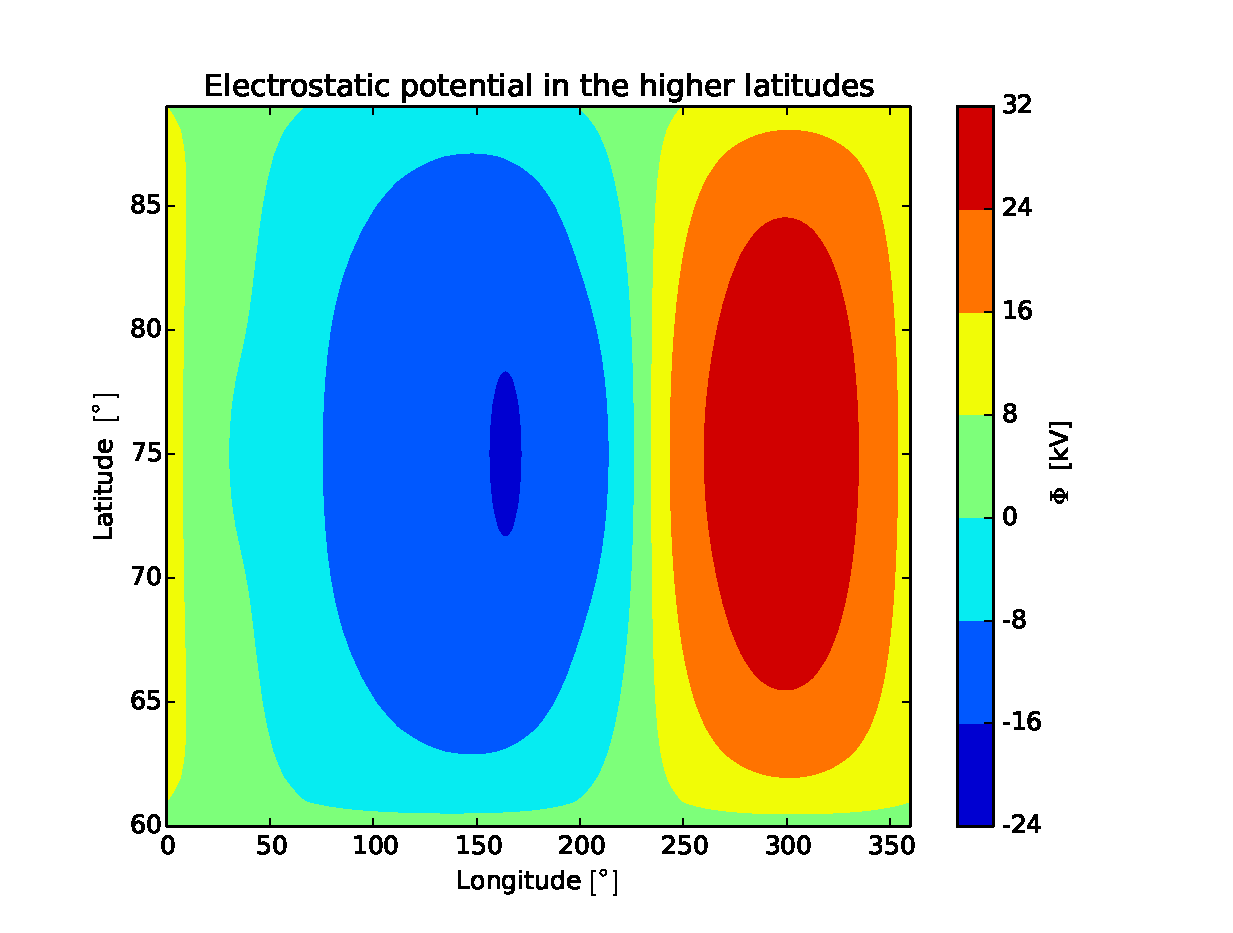
\includegraphics[width = \textwidth]{../source/potential}
        \subcaption{The figure shows the electrostatic potential in the higher latitudes, and the color indicates the magnitude of the potential compared to a reference value, with red being a high potential and blue being a low potential. One negative pole is located at \(150 \si{\degree}\) longitude and one positive at \(300 \si{\degree}\).}
      \end{subfigure}
      \hfill
      \begin{subfigure}{0.75\textwidth}
        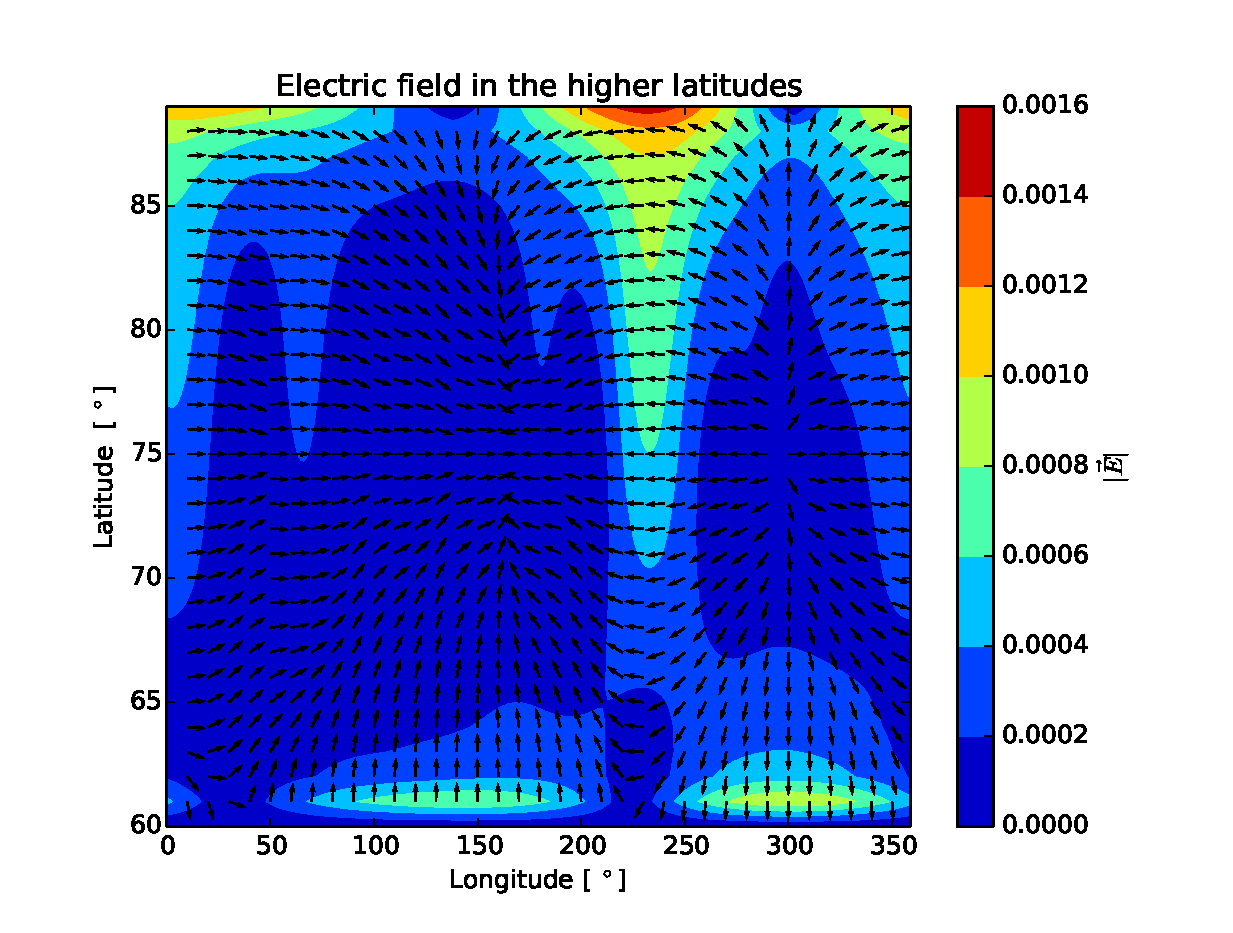
\includegraphics[width = \textwidth]{../source/eArrows}
         \subcaption{The figure shows the direction of the electric field, given by \(\va{E} = -\nabla\Phi\), in the higher latitudes and the magnitude, with the arrows showing direction and  the color representing magnitude. (Should probably use a dB scale for the strength)}
      \end{subfigure}
      \label{fig:pot_Electric}
    \end{figure}

    \begin{figure}
      \centering
      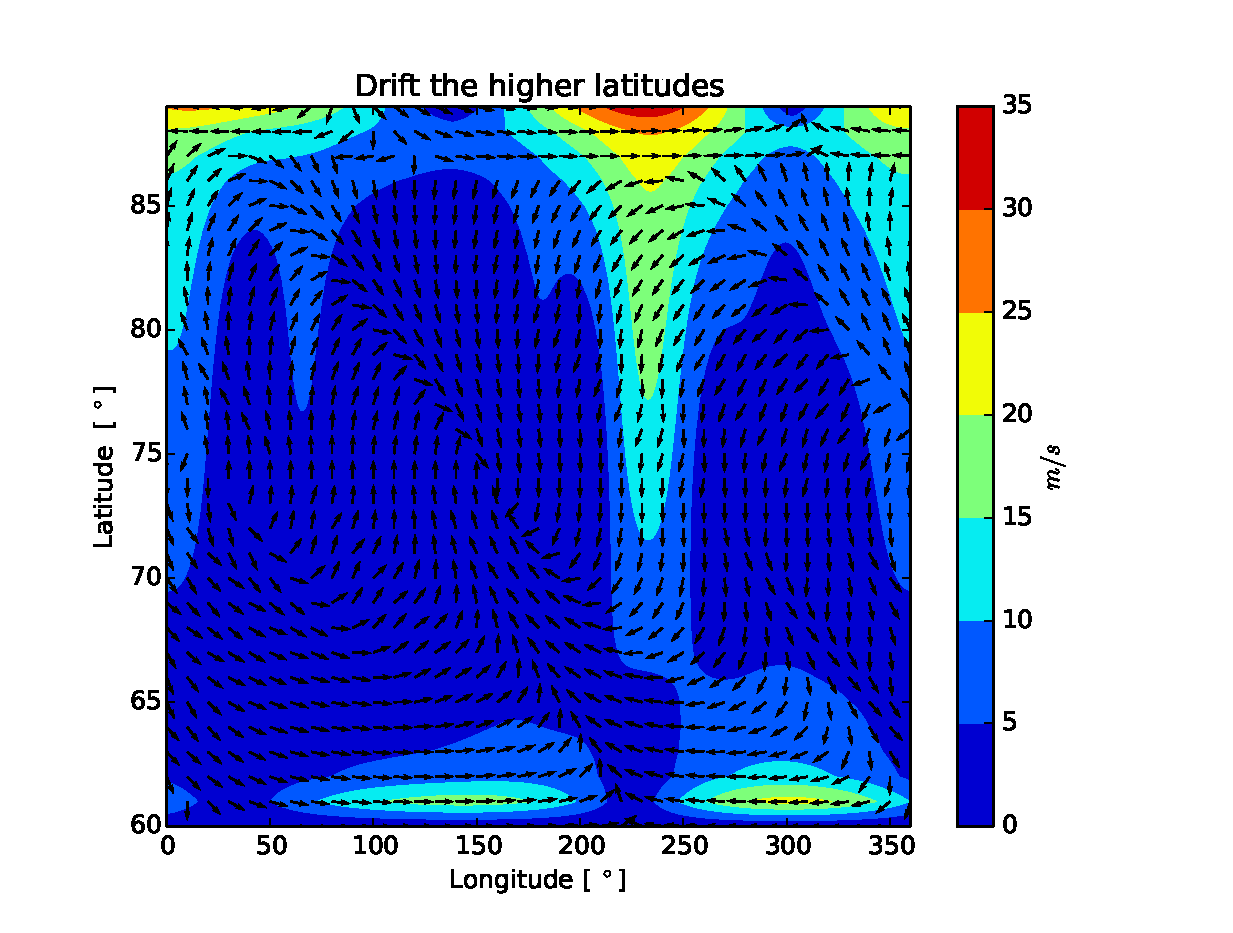
\includegraphics[width = \textwidth]{../source/vArrows}
      \caption{This shows the velocities direction and magnitude of the plasma caused by the E-cross-B drift. The scale of the drift is of an order \(1 \si{\meter\second}\)}
    \end{figure}


\appendix
\section{Comments regarding the exercise}
    \begin{itemize}
      \item A vertical magnetic field is meant along the z-axis? Could be compared to Earth's surface as well.
      \item What should be done with the edges of \(\nabla \Phi\)? Now I am ignoring them, but something like \( \pdv{\Phi_{0,j}}{\theta} = \frac{ \Phi_{0+1, j} - \Phi_{i, j} }{\Delta \theta}\) or similar methods could be implemented.
      \item Should we use \(r = Re\), that would be on the surface?
      \item If the mangetic field was meant to be vertical compared to the surface, is there an easier way to do the cross product? Than converting to cartesian, do the cross product and then converting back to spherical coordinates.
      \item Using the z-axis magnetic field there is also some drift in the radial direction, should that be there?
    \end{itemize}


\section{Code}
  \label{sec:code}
  \lstinputlisting{../source/convection.py}


\end{document}